\documentclass{article}
\usepackage{graphicx}
\usepackage{amsmath, amsfonts, mathtools}
\usepackage{amsthm}
\usepackage{todonotes}
\usepackage[ruled, linesnumbered]{algorithm2e}
\usepackage{enumerate}
\usepackage{float}
\usepackage{subcaption}
\usepackage{dsfont}
\usepackage{pythonhighlight}
\usepackage{listings}
\usepackage{xcolor}
\usepackage{xurl}
\usepackage{algorithm2e}
\usepackage{hyperref}
\usepackage[numbers]{natbib}

% Define colors for syntax highlighting
\definecolor{codegreen}{rgb}{0.2,0.6,0.2}
\definecolor{codegray}{rgb}{0.5,0.5,0.5}
\definecolor{codepurple}{rgb}{0.58,0,0.82}
\definecolor{backcolour}{rgb}{0.95,0.95,0.92}


% Sensible defaults for lstlistings
\lstset{
numberstyle=\tiny\color{codegray},
backgroundcolor=\color{backcolour},   
  basicstyle=\footnotesize\ttfamily,
  belowcaptionskip=1\baselineskip,
  breaklines=true,
  commentstyle=\bfseries\color{purple!40!black}
  frame=L,
  identifierstyle=\color{blue},
  keywordstyle=\bfseries\color{green!40!black},
  language=python,
  showstringspaces=false,
  stringstyle=\color{orange},
  xleftmargin=\parindent,
  captionpos=b,                    
    keepspaces=true,                 
    numbers=left,                    
    numbersep=5pt,                  
    showspaces=false,                
    showstringspaces=false,
    showtabs=false,
    tabsize=2,
    framexleftmargin=16pt,
    framextopmargin=6pt,
        framexbottommargin=6pt, 
        frame=tb, framerule=0pt,
}


\title{Approximation Algorithms - Assignment 4}
\author{Group 2: Christoph Kern, Johannes Gabriel Sindlinger}


\begin{document}

\maketitle

\noindent\fbox{\begin{minipage}{0.98\textwidth}
    \textbf{Task 1}\\
    Argue that for every triangle in the graph, it is valid to add an extra constraint requiring at least two vertices to be selected, in the sense that it does not remove any integer feasible solution. 
\end{minipage}}
\vspace{1em}

Let $G=(V,E)$ be some arbitrary graph and let $S$ be some vertex cover of $G$. Now suppose there exist a set of three distinct vertices $v_1, v_2, v_3 \in V$ such that $\{v_1, v_2\}, \{v_2, v_3\}, \{v_1, v_3\} \in E$, i.e.~$v_1, v_2$ and $v_3$ form a triangle. Since for every edge we must have one endpoint in the vertex cover, $v_1$ or $v_2$ must be in $S$ due to edge $\{v_1, v_2\}$.
\begin{itemize}
    \item Case $v_1 \in S$: Then either $v_2$ or $v_3$ is in $S$ due to edge $\{v_2, v_3\}$. 
    \item Case $v_2 \in S$: Then either $v_1$ or $v_3$ is in $S$ due to edge $\{v_1, v_3\}$. 
\end{itemize}

In any case, we have two vertices of $\{v_1, v_2, v_3\}$ in $S$. Since this was an arbitrary triangle in an arbitrary graph, it holds in general that two vertices of any triangle must be included in the vertex cover. Therefore, we can add this additional constraint to our IP formulation without removing feasible solutions.
\vspace{2.5em}

\noindent\fbox{\begin{minipage}{0.98\textwidth}
    \textbf{Task 2}\\
    Write code to add these constraints to the existing ones. You can modify the existing Python code, or build your own implementation from scratch in another language.
\end{minipage}}
\vspace{1em}

We will use the original \lstinline|APX| wrapper class to load the example graphs and use the LP implementation. In order to determine the degree of a vertex or to test if an edge is in the graph, we will use the graph data structure provided by \lstinline|NetworkX|. The following function \lstinline|load_graph| loads a graph into memory:

\begin{lstlisting}
def load_graph(filename):
  graph = nx.Graph(name=filename)
  for e in DataFile(filename):
    graph.add_edge(*e)
  return graph
\end{lstlisting}

We will also use the same mechanism for rounding the solution as in the provided python code. For better readability, we moved this segment into its own function \lstinline|round_solution|:

\begin{lstlisting}
def round_solution(solution):
    rounded_value, rounded_solution = 0, {}
    for x, v in solution.items():
        r = int(np.round(v + 1e-10))
        rounded_solution[x] = r
        rounded_value += r
    return rounded_value, rounded_solution
\end{lstlisting}

Finally, the function \lstinline|vertex_cover_lp| creates the LP-relaxation of the integer program intended to solve the vertex cover problem for the given graph. With the flag \lstinline|triangle_constraints|, we can decide whether we want to add the suggested triangle constraints to the formulation or not. The triangles are computed using the \textsc{MinBucket} algorithm described by \citet{Berry15}. The implementation of \lstinline|vertex_cover_lp| looks as follows:

\begin{lstlisting}
def vertex_cover_lp(graph, triangle_constraints=False):
  lp = LinearProgram('min')
  buckets = {}
  objective = {}
  
  for v in graph.nodes():
    objective[v] = 1.0
    buckets[v] = []
  
  for (u,v) in graph.edges():
    lp.add_constraint({u: 1, v: 1}, 1)
    if graph.degree[u] <= graph.degree[v]:
      buckets[u].append(v)
    else:
      buckets[v].append(u)
          
  if triangle_constraints:
    for u, bucket in buckets.items():
      for (v,w) in combinations(bucket, 2):
        if graph.has_edge(v, w):
          lp.add_constraint({u: 1, v: 1, w: 1}, 2)
      
  lp.set_objective(objective)
  return lp
\end{lstlisting}

\begin{itemize}
    \item Lines 2-4: Initialize the LP, create a dictionary for storing the buckets, and create a dictionary that represents the objective. 
    \item Lines 6-8: Creates the objective function and creates an empty bucket for each vertex.
    \item Lines 10-15: Creates constraint that expresses that for each edge $\{u,v\}$, at least one endpoint must be in the vertex cover. Furthermore, if $d_u \le d_v$, we add $v$ to the bucket of $u$, otherwise we add $u$ the the bucket of $v$.
    \item Lines 17-21: If we decide to add the triangle constraints, for each bucket we look at each wedge and check whether there is an edge completing the triangle. If a triangle is found, we add a constraint that expresses that at least two of the vertices of the triangle must be in the vertex cover. 
\end{itemize}

To finally test the implementation on all provided example graphs, we run following code with some additional print statements (not shown here):
\begin{lstlisting}
for filename in DataFile.graph_files:
  graph = load_graph(filename)
  
  lp = vertex_cover_lp(graph)
  value, solution = lp.solve()
  rounded_value, rounded_solution = round_solution(solution)
  
  lp_t = vertex_cover_lp(graph, triangle_constraints=True)
  value_t, solution_t = lp_t.solve()
  rounded_value_t, rounded_solution_t = round_solution(solution_t)
\end{lstlisting}

The full implementation can be found on \url{https://github.com/chrisiKern/Approximation-Algorithms-2024/blob/main/Assignment4/Vertex_cover.ipynb}.
\vspace{2.5em}

\noindent\fbox{\begin{minipage}{0.98\textwidth}
    \textbf{Task 3}\\
    Compare the rounded solutions, as well as the lower bounds on the optimal solution, to the original implementation.
\end{minipage}}
\vspace{1em}


Recall that the solution of the LP-relaxation of the integer program expressing the vertex cover problem only gives us a lower bound on the optimal solution. With the rounding procedure, we obtain a solution of the integer program that gives us a valid vertex cover, but it may not necessarily be optimal. Following table shows the corresponding objective function values with and without the additional triangle constraints for each of the provided graphs.

\begin{center}
    \begin{tabular}{l|r r|r r}
        \multicolumn{1}{c}{\textbf{Graph}} & \multicolumn{2}{|c|}{\textbf{Basic}} & \multicolumn{2}{c}{\textbf{+ Triangles}}\\
        & Value & Rounded & Value & Rounded\\
        \hline
        \lstinline|routes.txt| & 5.00 & 10 & 6.00 & 6\\
        \lstinline|petersen.txt| & 5.00 & 10 & 5.00 & 10\\
        \lstinline|petersenstar.txt| & 6.00 & 11 & 6.00 & 11\\
        \lstinline|star.txt| & 1.00 & 1 & 1.00 & 1\\
        \lstinline|clique.txt| & 2.50 & 5 & 3.33 & 5\\
        \lstinline|cycles.txt| & 3.50 & 5 & 4.00 & 4\\
        \lstinline|lotr.txt| & 31.50 & 50 & 37.67 & 49\\
        \lstinline|karate.txt| & 13.50 & 16 & 14.00 & 14\\
        \lstinline|noisybiclique.txt| & 21.00 & 42 & 28.00 & 42\\
    \end{tabular}
\end{center}

First, let us consider the obtained objective function values of the LP-relaxation with and without the triangle constraints, i.e.~lower bounds of the optimal solution. As expected, the formulation with the triangle constraints gives us a tighter lower bound than the formulation without them for almost all graphs. Only for \lstinline|petersen.txt|, \lstinline|petersenstar.txt|, and \lstinline|star.txt| there is no improvement. However, this is not surprising as neither of these graphs contain triangles. Thus, the LP formulations are identical and, therefore, we obtain identical results.

Considering additionally the objective function value of the rounded solutions, we also see significant improvements for the formulation with triangle constraints over the original version. Apart from the instance above, only \lstinline|clique.txt| and \lstinline|noisybiclique.txt| do not yield an improvement. Since \lstinline|clique.txt| is a clique of 5 vertices, any vertex cover must contain those 5 vertices, so this is expected. For \lstinline|noisybiclique.txt|, both solutions contain all vertices, but we are not sure if this is strictly necessary in any solution.

There are also several instances where we actually found the optimal solution. This is the case when the value of LP-relaxation matches the value of the rounded solution. For \lstinline|star.txt| this was the case for both the formulation with the triangle constraints and without. Furthermore, we also found the optimal solution for \lstinline|routes.txt|, \lstinline|cycles.txt|, and \lstinline|karate.txt| with the help of the additional constraints. 

As an example where the additional constraints significantly improved the solution (and actually enabled us to find the optimal solution), was \lstinline|routes.txt|, shown in Figure~\ref{fig:routes}. We can see that it contains a lot of triangles, thus a lot of triangle constraints were added.

\begin{figure}
    \centering
    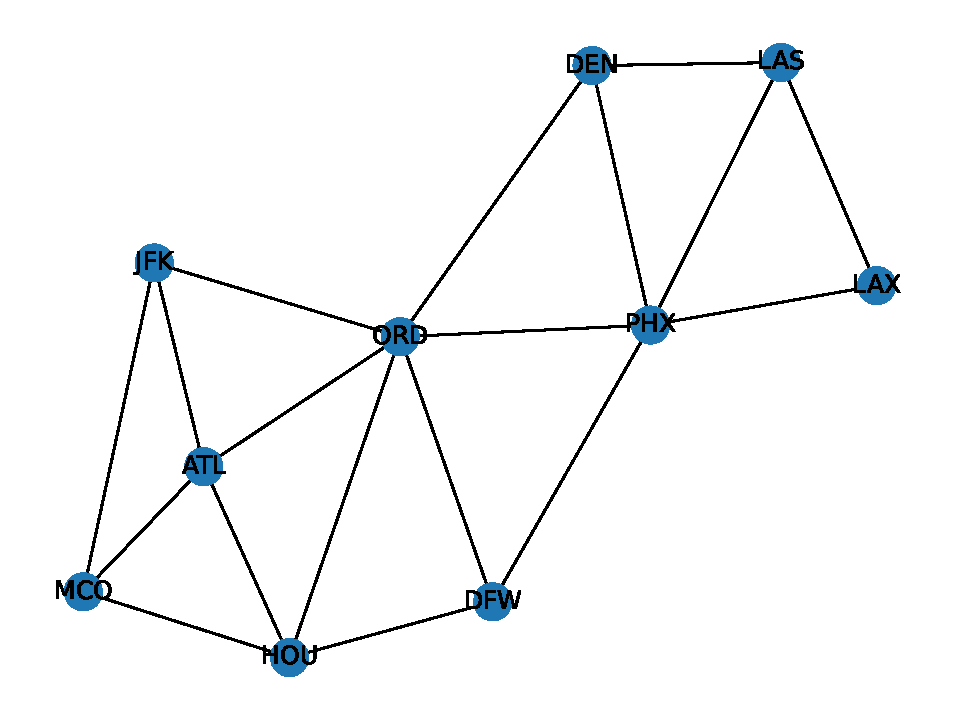
\includegraphics[width=.8\linewidth]{Assignment4/routes.pdf}
    \caption{Visualization of the graph \lstinline|routes.txt|}
    \label{fig:routes}
\end{figure}

\begin{lstlisting}
Without triangle constraints:
	- Solution: {'JFK': 0.5, 'MCO': 0.5, 'ATL': 0.5, 'ORD': 0.5, 'HOU': 0.5, 'DEN': 0.5, 'DFW': 0.5, 'PHX': 0.5, 'LAS': 0.5, 'LAX': 0.5}
	- Rounded: {'JFK': 1, 'MCO': 1, 'ATL': 1, 'ORD': 1, 'HOU': 1, 'DEN': 1, 'DFW': 1, 'PHX': 1, 'LAS': 1, 'LAX': 1}
With triangle constraints:
	- Solution: {'JFK': 0.0, 'MCO': 1.0, 'ATL': 1.0, 'ORD': 1.0, 'HOU': 0.0, 'DEN': -0.0, 'DFW': 1.0, 'PHX': 1.0, 'LAS': 1.0, 'LAX': 0.0}
	- Rounded: {'JFK': 0, 'MCO': 1, 'ATL': 1, 'ORD': 1, 'HOU': 0, 'DEN': 0, 'DFW': 1, 'PHX': 1, 'LAS': 1, 'LAX': 0}

\end{lstlisting}





\bibliographystyle{plainnat}
\bibliography{bibliography}

\end{document}
